%7.8
Vi bruker den numeriske løsningen til $\phi_2$ langs svømmeflaten $S_B$ for å regne addert masse $a_{22}$ og dempning $b_{22}$ for bølgetall (ganget med dypgang) fra 0 til 2: $0 < KD = \omega D / g < 2$. Vi regner også ut $b_{22}$ fra energibalansen. %Altså gjennomsnittlig energifluks og ..?
(merk: subscript 2 midlertidig fjernet for $\xi, A, amp$)
\begin{align}
	\frac{1}{2} |\xi|^2 \omega^2 b_{22} &=  {\bar{E}^{\infty} c_g + \bar{E}^{-\infty} c_g }\\
	%
	b_{22} &=  \frac{\bar{E}^{\infty} c_g + \bar{E}^{-\infty} c_g }{\frac{1}{2} |\xi|^2 \omega^2}\\
	%visual spacing for myself to read
	b_{22} &=  \frac{\cancel{\frac{1}{2}}\rho g |amp^{\infty}|^2  c_g + \cancel{\frac{1}{2}}\rho g |amp^{-\infty}|^2 c_g }{\cancel{\frac{1}{2}} |\xi|^2 \omega^2}\\
	%spacing
	b_{22} &=  \frac{ \rho g |amp^{\infty}|^2  (\frac{g}{2\omega}) +  \rho g |amp^{-\infty}|^2 (\frac{g}{2\omega}) }{ |\xi|^2 \omega^2}\\
	%spacing
	b_{22} &=  \frac{\rho g {|\xi A^{\infty} \frac{\omega^2}{g}|}^2  (\frac{g}{2\omega}) +  \rho g {|\xi A^{-\infty} \frac{\omega^2}{g}|}^2  (\frac{g}{2\omega}) }{ |\xi|^2 \omega^2}\\
	%
	b_{22} &=  \frac{  \rho g \cancel{|\xi|^2} (\frac{\color{red}{\omega^2}}{g})(\frac{\omega^2}{g}) {| A^{\infty} |}^2  (\frac{g}{2\omega}) + \rho g \cancel{|\xi|^2}  (\frac{\color{red}{\omega^2}}{g})(\frac{\omega^2}{g}) {| A^{-\infty}|}^2  (\frac{g}{2\omega}) }{ \cancel{|\xi|^2} \color{red}{\omega^2}}\\
	%
	b_{22} &=   \rho  \cancel{g  (\frac{1}{g})}(\frac{\omega^2}{g}) {| A^{\infty} |}^2  (\frac{g}{2\omega}) +  \rho \cancel{g   (\frac{1}{g})}(\frac{\omega^2}{g}) {| A^{-\infty}|}^2  (\frac{g}{2\omega}) \\
	%
	b_{22} &=  \rho  (\frac{\omega^2}{g})   (\frac{g}{2\omega}) ({| A^{\infty} |}^2 +  {| A^{-\infty}|}^2)\\
	%
	b_{22} &=    \frac{1}{2} \rho \omega ({| A^{\infty} |}^2 +  {| A^{-\infty}|}^2)
\end{align}
Legger på subscript og flytter omega og rho under, så får vi ønsket likning, 
\begin{align}
	\frac{b_{22}}{\rho \omega} &=    \frac{1}{2}  ({| A_2^{\infty} |}^2 +  {| A_2^{-\infty}|}^2)
\end{align}

\subsection{Vi ser på addert masse og sammenlikner de to fremgangsmåtene for å finne $b_{22}$}

\noindent
\begin{minipage}[t]{0.45\linewidth}
    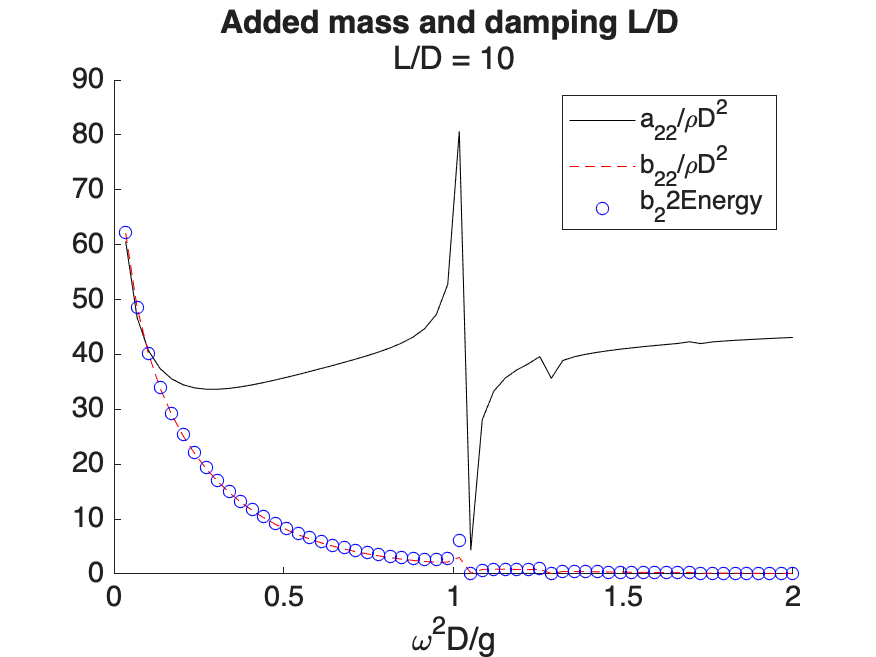
\includegraphics[width=\linewidth]{/Users/ole/Tex/MEK4420/oblig2images/plot_a22b22_1.png}
    \captionof{figure}{L/D = 10}\label{fig:a22_1}
\end{minipage}
\hspace{0.05\linewidth}
\begin{minipage}[t]{0.45\linewidth}
    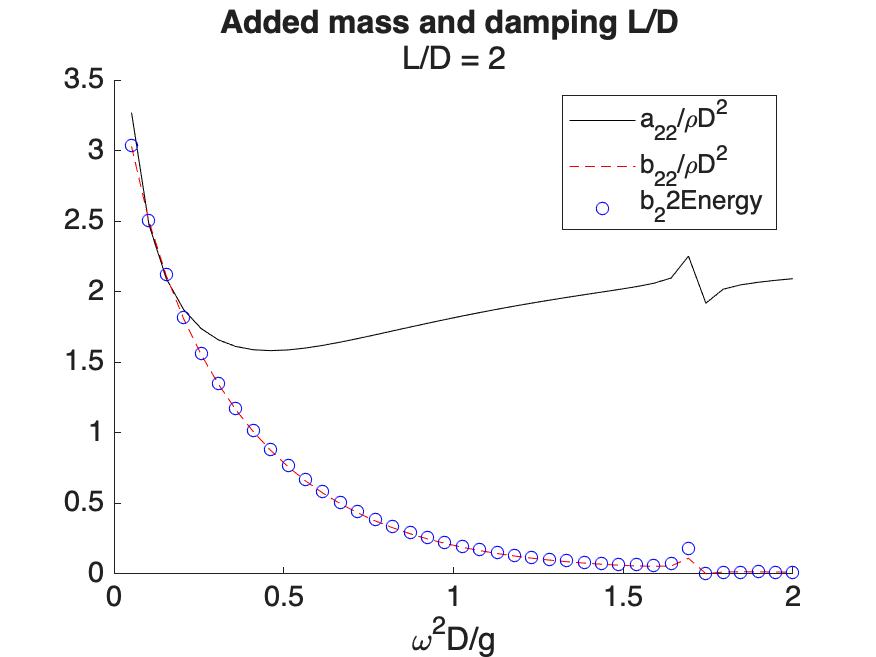
\includegraphics[width=\linewidth]{/Users/ole/Tex/MEK4420/oblig2images/plot_a22b22_2.png}
    \captionof{figure}{L/D = 2}\label{fig:a22_2}
\end{minipage}

\vspace{0.5cm} % Adds vertical space between rows

\noindent
\begin{minipage}[t]{0.45\linewidth}
    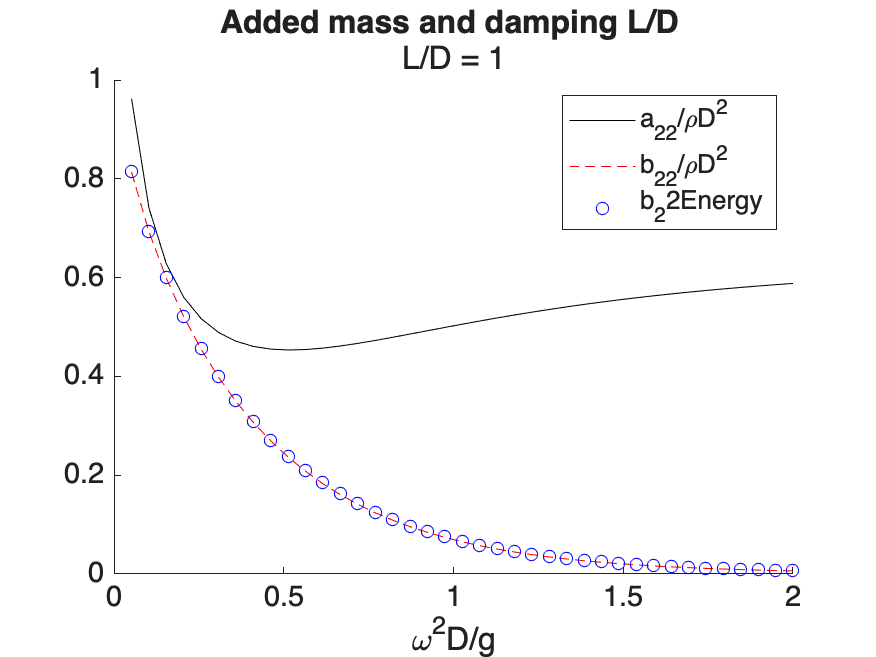
\includegraphics[width=\linewidth]{/Users/ole/Tex/MEK4420/oblig2images/plot_a22b22_3.png}
    \captionof{figure}{L/D = 1}\label{fig:a22_3}
\end{minipage}
\hspace{0.05\linewidth}
\begin{minipage}[t]{0.45\linewidth}
    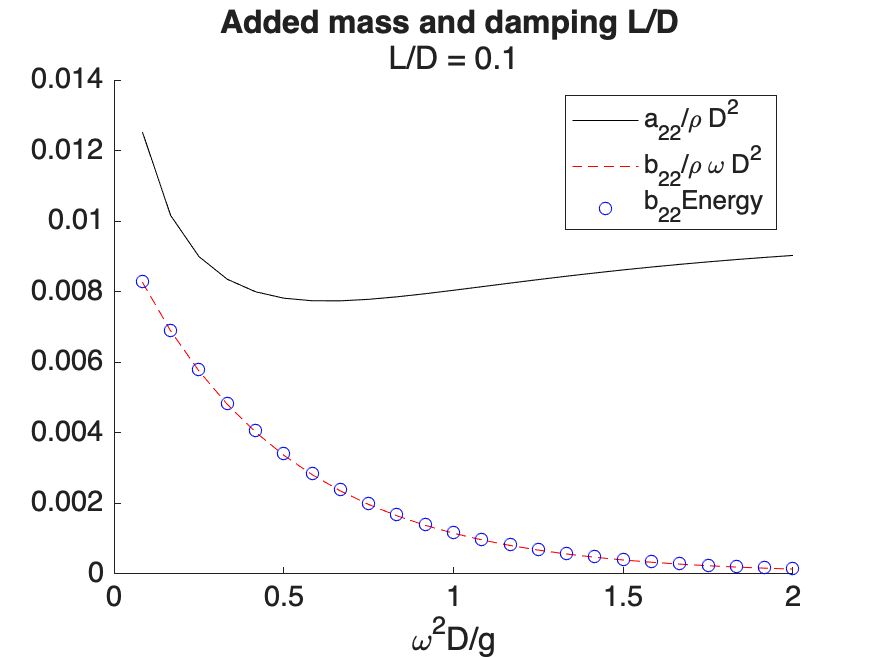
\includegraphics[width=\linewidth]{/Users/ole/Tex/MEK4420/oblig2images/plot_a22b22_4.png}
    \captionof{figure}{L/D = 0.1}\label{fig:a22_4}
\end{minipage} 